\documentclass[oneside]{book}
\usepackage{xcolor}
\definecolor{bg}{rgb}{0.95,0.95,0.95}
\definecolor{emphcolor}{rgb}{0.5,0.0,0.0}
\newcommand{\empha}{\bf\color{emphcolor}}
\usepackage{parskip}
\usepackage{minted}
\usepackage{caption}
\usepackage{amsmath}
\usepackage{amssymb}
\usepackage{amscd}
\usemintedstyle{friendly}
\setminted{bgcolor=bg,xleftmargin=15pt}
\usepackage{hyperref}
\hypersetup{pdftex,colorlinks=true,allcolors=blue}
\usepackage{hypcap}
\usepackage{graphicx}
\title{Communicating Sequential Processes\\ in C++}
\author{John Skaller}
\begin{document}
\maketitle
\tableofcontents
\chapter{CSP model}
The CSP kernel supports a simple architecture. It is based on a scheduler mediated
continuation passing model. A continuation is an object encapsulating execution
state in a form where if running it can be suspended in such a way execution
can be resumed.

\section{Systems}
A {\em system} consists of several {\em processes} which communicate
using {\em asynchronous channels}. Systems are used to manage 
core {\em internal} resources: processing elements (CPUs), program code,
time, and data memory.

A {\em device} is an arbitrary object and associated service thread which is
used to manage {\em external} resources, including network and file system access,
and user interfaces.


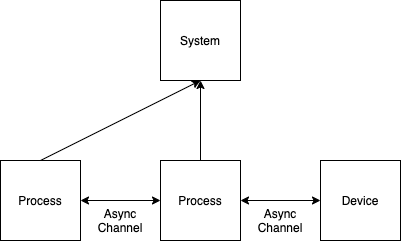
\includegraphics{../src/tex/system.png}

Processes within the same system can communicate with each other or
with devices. Processes in distinct systems must use a device as
a middleman to communicate.

\section{Processes}
The execution of a process is effected by one or more {\em threads}.
If there is only one, the process is {\em single threaded,} otherwise
if there are two or more, {\em multi-threaded.} Every process is started
with a single {\em initial} thread.

A {\em fibre} is a logical thread of control and associated execution
context. Each process consists of a collection of fibres. 

Fibres in a process are {\em running} if a thread is elaborating the
fibre's program code, otherwise the fibre is {\em suspended}. 

A suspended fibre can either be {\em ready} or {\em waiting}.
The collection of ready and running fibres are said to be {\em active}.

All the ready fibres of a processes are maintained in a set and
are owned by their process. Running fibres are owned by the thread
running them which are owned by the thread's process.

When a thread is out of work, it attempts to locate a 
ready fibre then run it. If there are no ready fibres,
no fibres are running, and there are no fibres waiting on
asynchronous I/O from an external device or another system,
then the process terminates and all associated memory is released,
all but the initial thread are terminated, and the initial thread
returns control.

A process is initiated by a single C++ function call
which is passed a pointer to an initial fibre suspension to invoke
and a pointer to the owning system. A single threaded processes
is then constructed with a single fibre owning the initial 
fibre.

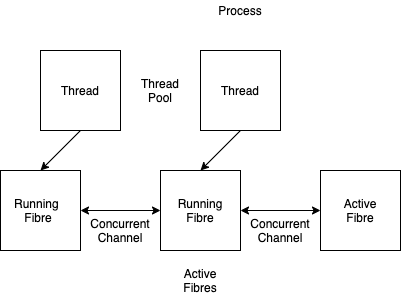
\includegraphics{../src/tex/process.png}


\section{Fibres}

A {\em fibre} consists of a stack of continuations.

\subsection{Continuation Objects} 
A {\em continuation object} is an instance of a routine. Continuations can
be {\em suspended} and {\em resumed.} Suspension is always the result
of the action of the routine itself: there is no premptive suspension.

Continuations are instances of a the
abstract type \verb%con_t% which has a \verb%resume()% method.
Calling this method continues execution of the continuation,
whilst returning from it leaves it in a suspended state so
that (if correctly programmed) the next invocation of the
resume method continues execution from the suspension point
with the data state of the continuation the unchanged, except
possibly if a channel I/O service call completed or a subrouine
returned a value.

\subsection{Coroutines}
There are two kinds of routine. A {\em coroutine} representes the type
of the initial routine of a fibre. An instance of a coroutine must be
{\em spawned} by a service call which yields a fibre with one continuation
on its stack. Coroutines are typically infinite loops and they cannot 
logically return control, for there is nowhere to return to. They can,
however, terminate by {\em suicide.}

\subsection{Subroutines}
A {\em subroutine} represents the type of a routine which can be invoked
by a {\em call} operation in a way analogous to subroutines in a 
convential stack machine. A call pushes the instance onto the fibre stack
suspending the caller and running the subroutine continuation, which is 
prepared to start at its entry point.



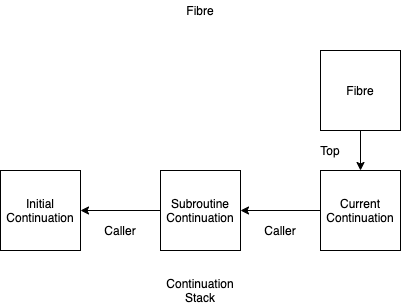
\includegraphics{../src/tex/fibre.png}

\section{Channels}

A {\em channel} is a synchronisation primitive which also allows transmission
of data.

Channels are accessed via {\em channel endpoints}, using {\em channel endpoint references.}

A particular channel enpoint may be accessed only from the continuations
of one fibre; that is, each endpoint must be uniquely owned by a single
fibre. This invariant ensures the correct termination of fibres
making I/O requests which cannot be satisfied. 

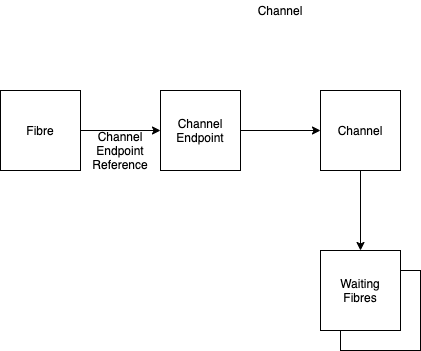
\includegraphics{../src/tex/channel.png}

\chapter{Access}
Objects in the system can access others using either pointers
or reference counting smart pointers. A variable containing a pointer
which expresses ownership is called a {\em strong pointer variable}.
Reference counting pointer variables are always strong.

Ordinary pointers can also be strong. In this case, the object referred
to must be manually deleted before the object containing the variable
is destroyed.

A weak pointer variable is a variable containing a pointer which provides
access to an object which owns, directly or indirectly, the containing
variable. Such objects must be deleted before the owning object is deleted
so that the lifetime of the weak pointer variable is contained temporally
in the owner lifetime.

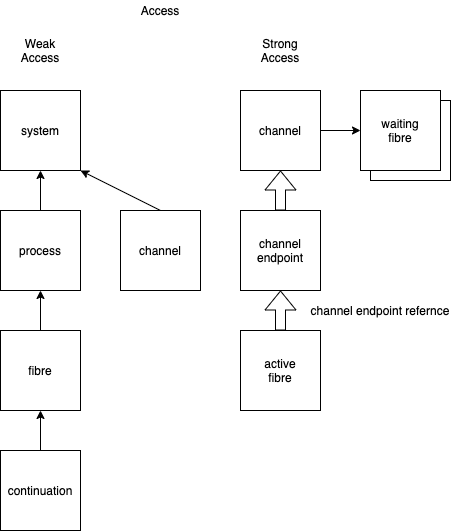
\includegraphics{../src/tex/weak_access.png}

\chapter{Operational Semantics}
The core semantic operations of the system are construction of
processes, threads, and fibres, and channel I/O.

\subsection{Termination}
The termination semantics of our CSP model are novel. A correctly constructed
system cannot deadlock. Instead, the system is guarranteed
to terminate if, and only if, there is no work being done, and no possibility
of further work appearing.

When a single thread is idle but other threads are running, the running jobs
can generate new work which may be taken up by the idle thread. So an idle
thread must wait in this case.

If there is no work for any thread, but an async operation is pending,
further work will be created when the suspension awaiting the async
operation is resumed, so again, no threads may terminate.

Otherwise, the system terminates. This model has two distinct problems.



\section{Channel Semantics}
Reads and writes on channels are performed with special service calls
which are given a channel endpoint reference. The semantic rules
are simple enough.

A channel may be in three states. It may be empty, consist of a set
of readers, or consist of a set of writers.

\subsection{Write Semantics}
When a write is performed then, if the channel is empty or consists 
of a set of writers, the fibre performing the write is added to the channel.
Since this fibre we the currently running fibre of some thread, and the
fibre is now suspended, the thread no attempts to find another 
fibre to execute.

If the channel contains a reader then, instead, it is removed from
the channel. Data is transfered from the writer to the reader.
Nominally, both fibres then become active fibres of their 
respective processes.

\subsection{Read Semantics}
Dual to write semantics except the direction of data transfer is the same
in both cases, from writer to reader.


\subsection{Channel types}
There are three types of channels.

\subsubsection{Sequantial Channel}
Always safe in a single threaded system lacking asynchronous I/O,
this kind of channel has the fastest operation.

\subsubsection{Concurrent Channel}
This kind of channels works the same way as a sequential
channel but a spinlock is used to protect the critical part
of the operations. It is always safe between fibres of the same system.

\subsubsection{Asynchronous Channel}
This kind of channel must be used to communicate with external devices.

First, a device must send a signal to a process when it completes an I/O
operation. Completion of an I/O operation causes a suspended fibre to
become active and the signal is required to wake up any sleeping threads
so allow the fibre to be resumed.

Second, a fibre must send a signal to a device when it initiates
an I/O operation, to wake up the device management thread in
case it is sleeping, to process the I/O request.

The action of a device is not arbitrary. On completing an I/O request
it must push the requesting fibre back onto the process active set
and then issue the required signal. However the precise action
of the device thread apart from this is dependent on the nature
of the device.

\section{Sequential Model}
A closed process with a single thread can be implemented using sequential channels,
it has the simplest semantics and highest performance because no inter-thread synchronisation
is required.

In a sequential system a single thread executes a routine whilst a set of other 
routines are suspended.

When a fibre terminates, a suspension is fetched from the active set and
resumed, unless there are none, in which case the scheduler returns to its caller
and the CSP subsystem is terminated.

There are four operations a fibre can perform which impact fibre scheduling.

\begin{itemize}

\item{Suicide} The fibre terminates. The scheduler runs another active fibre or terminates
if there are none.

\item{Spawn} The fibre creates a new active fibre. The current and newly constructed
fibre are active. The scheduler may run any active fibre. Our implementation provides
two service calls, one which continues running the current fibre, suspending the
new one, and one which suspends the current fibre and runs the new one.

\item{Read/Write} A fibre performs a read or write operation on a channel.
A detailed description is below.

\end{itemize}

\subsection{Channel I/O}
A fibre performing a read on a channel is called a reader. A fibre performing
a write is called a writer. A read operation is said to match a write.

A channel is a set of fibres, possibly empty, all of which are
readers or all of which are writers.

If a channel consists of a non-empty set of readers a write operation will succeed.
It is performed by removing one reader from the set, transfering a machine word
from the writer to the reader, and making both reader and writer active.

Similarly a read operation will succeed if the channel consists of a non-empty
set of writers. It is performed by removing one writer from the set, transfering
a machine word from the writer to the reader, and making both reader and writer active.

In our implementation in a sequential system the reader is always resumed and the
writer suspended so the reader "goes first" and may use the opportunity to copy
data from the writer before the writer has a chance to modify it, however the
abstract semantics do not specify this, and concurrent and asynchronous channel
operations cannot ensure this.

If the channel is empty or an I/O operation does not find a matching fibre
in the channel, then there exists a channel endpoint which might be used
later to satisfy the I/O request, the requesting fibre is suspended and
added to the channel, and the scheduler then picks another fibre to run.

Otherwise, if the only remaining channel endpoint is the one being
used to perform the I/O request, there is no possibility that the
I/O operation can succeed. In this case, the channel, along with all
fibres suspended on it, is deleted, the caller fibre is deleted,
and the scheduler now looks to find another fibre to run from
the active set. Crucially, if no such fibres exist, the scheduler
terminates and returns control to its caller.

A reader waiting on a matching write is said to be {\em hungry,}
a writer waiting on matching read is said to be {\em loaded.}
If a fibre is hungry and no matching write will be performed
the fibre is said to be starved. If a fibre is loaded and no
matching read will be performed, the fibre is blocked.

In a correctly constructed system, a fibre which is starved because there is no
endpoint on which a write could be performed is deleted and so
such fibre cannot exist. Similarly a fibre which is blocked
and for which no endpoint exists which could be used to
peform a read, is deleted and so cannot exist.

A correctly constructed system must satisfy the constraint that
no fibre can access more than one endpoint of the same channel.
Note this rule may be transiently broken during construction
by an initialisation routine.

Deadlocks may still occur. In the simplest case a fibre A
reads on channel 1 and then writes on channel 2, whilst a fibre
B reads on channel 2 then writes on channel 1. Fibre A is suspended
on the channel 1 read operation and fibre B is suspended on the
channel 2 read operation. Each fibre holds an endpoint for the channel
on which the other is waiting, so the termination condition is not met
and the system is deadlocked. [Note this cannot happen in the garbage
collected version of Felix because the collector performs exhaustive
reachability analysis.)

The algorithm used to implement I/O is novel. We use three objects,
and double indirection with reference counting.

Each channel has a set of associated endpoints, a count of which
is maintained in the channel. The endpoints in turn are accessed
by a dedicated shared pointer type which manages a reference count
stored in the endpoint.

When there are no references to an endpoint, the endpoint is
deleted and the count of endpoints in the channel decremented.
If the count would become zero, the channel, and all fibres
waiting for I/O on that channel deleted.

However, when an unmatched read or write is performed on a channel
and the reader or writer fibre would normally be added to the channel,
the reference count in the channel is also decremented, and, when a
fibre is removed from a channel due to a matching I/O operation,
the count is incremented.

Thus, the reference count mainted in the channel is not a count
of the number of endpoints in existence but rather the number
of endpoints which are owned by fibre not suspended on the channel.
Note that this does not allow for a fibre suspended on another channel,
which is why a deadlock can occur.

If the reference count of the channel is one and would become
zero, the channel is deleted along with the fibre requesting
the I/O operation and all the fibres suspended on the channel.

Note carefully this deletion process is recursive and potentially
circular: deleting a channel deletes all the fibres on it which
destroys all endpoint references held by these fibres which
in turn can delete endpoints of other channels and thus also
those channels, then recursively deleting all the fibres
of those channels.

The algorithm takes care to prevent infinite loops by marking
a channel being deleted by setting the reference count to 0
to indicate deletion is already in progress.

In most systems coroutines are infinite loops which repeatedly
process elements of data streams. The simplest configuration is
a pipeline consisting of a data source, a sequence of transducers,
and a terminal sink. In such a pipeline if any one of the components
suicides, the whole pipeline automatically collapses. 

This is the correct way for CSP systems to terminate. It must be repeated,
that blockage and starvation are not errors, but the correct method of termination.
That this is not the case in Golang is a fundamental design fault in that
system. It is important to note that it is impossible to check for
end of data on a channel: being able to do so actually makes the semantics
unsound.

We note again the Felix garbage collected implementation is more exhaustive.
It detects deadlocks too, so in a correctly constructed Felix system
deadlocks are impossible and simply lead to termination. Although our
system could also implement this capability, maintaining a data structure
representing all channels a fibre can access is potentially expensive
and may prohit the temporal bounds required for hard real time systems:
in particular the kernel would need to perform arbitrary allocations.
By contrast the existing system uses only linked lists of fibres,
where fibres have a slot for the next pointer, and so the kernel operation
itself requires no allocations at all.

\section{Concurrent Systsms}
A system can use pool of threads to execute more than one active
routine at once. All systems begin single threaded and the initial
thread is called the main thread. All threads are detached and terminate
by returning control; the main thread returns to its caller, whilst
the other threads, called {\em cothreads}, simply evaporate.

A routine can spawn a routine as a cothread. This adds a new thread
to the thread pool. Since more than one thread can now be running,
channel I/O requires inter-thread synchronisation. We use spinlocks
to achieve this because I/O operations are extremely light.

If the spinlocks also ensure no premption is possible whilst a thread
holds a lock, then the system would be lock free. Unfortunately most
operating systems do not provide non-premptable critical sections.
This means if there is heavy contention, and an I/O operation is prempted
whilst holding a lock, other thread will spin until the pre-empted thread
is resumed by the operating system.

This situation can be avoided on Linux if the thread has exclusive use
of a CPU core so that pre-emptions are not possible. It is also the
expected behaviour if heavy weight operating system mutex had been used,
although most operating systems to not ensure this. Unfortunately,
acquiring mutex locks is almost certainly involved in de-scheduling
threads attempting to acquire an already held lock, which no assurance
such a thread will be rescheduled rapidly after the lock is released;
so although the semantics may be superior real time performance
may be compromised.

This is because again most operating systems refuse to clearly specify
the meaing of real time assurances given to a thread, in the event
the thread performs come service call to the operating system: in principle
the time during which the service is performed should not be debited
from the temporal quota the thread has been issued (althougth the costs of
the call itself may be).

Operating systems do assure real time threads of their quotas if the
behave nicely, even if pre-empted: the time lost to a pre-emption
must be made up later. 

In addition, the lack of hardware synchronisation primitives is a severe
limitation on which can be achieved. Most processors provide atomic
versions of basic operations on a machine word, such as increment,
along with a CAS (compare and swap) instruction. Unfortunately CAS
along is next to useless. Even with DCAS (double compare and swap)
a simple stack cannot be implemented. What is actually required
is the ability to perform an short sequence of a reasonable selected
set of instructions atomically, as can be achieved with a non-preemptable
spinlock. 

\subsubsection{Idleness}
When multiple threads are able to pull jobs out of a job queue,
there is an issue what to do when there are no jobs in the queue.
If there are no currently running fibres at all, the system must
terminate.

On the other hand, if one job is running, we do not want to terminate
the idle threads, because the running fibe can spawn new work.
This means an idle thread should wait on a condition variable which
is signalled when either new work becomes available or, it is time
for all threads to return.

When a thread has no work, the cost of the OS calls required to
wait on a condition variable can be ignored, since the thread
has no work anyhow. However signaling all threads every time
a new job is spawned is not a good idea either: although we expect
and indeed demand signalling to be a real time operation, in practice
it may not be. We must therefore at least limit signaling to when it
is necessary.

A signal must be sent when there is at least one idle thread and the 
spawn operation is adding to an empty job queue. These conditions
are logically connected. However the emptiness of the job queue
is indicated by a nulptr, and we have to maintain a count of 
active threads and idle threads separately to allow termination.

The problem here is a potential race condition. Signally a thread
to wake up and grab a job off the queue does not ensure the job
is still there when the thread wakes up. On the other hand if
a thread is idle when a job is added to the queue, failing to
signal the thread just because the queue was not empty could
lead to a situation when a job is pulled off the queue by another
thread, leaving a job still waiting, but the idle thread was
not signalled.

In the end, a simple solution to this problem is to use a timed wait
on a condition variable. An idle thread simply polls for work or the
termination condition, with the option of being woken up by a signal
to reduce the delay in starting a job. This is a universal solution,
and the argument for it is simple enough: the thread is idle anyhow,
so the polling interval is chosen as a tradeoff between latency and
energy consumption.

\section{Asynchronicity}
So far we have dealt with closed systems. Although multithreaded
applications require synchronisation of channel I/O, the delays
are very small.

Asynchronous I/O involves waiting potentially long periods for
external events such as alarm timeouts, user interface inputs,
socket I/O, video sync pulses, audio callbacks, or communication
between distinct processes.

In this situation, fast polling by waiting threads is not acceptable.

We represent an external device as a thread which monitors actual hardware.
These threads are custom designed in an arbitrary manner. For example
socket I/O would use operating system dependent polling of event queues
by use of functions like poll, epoll, kqueue, etc to wait for
socket events.

Our system routines never block directly waiting for asynchronous events.
Instead, a fibre is simply made inactive in the same way as an unsatisfied
channel I/O request removes the fibre from the active set. When the 
wait is over some work is done by the device threads preparing the
fibre for resumption and then it is put back in its owning active set.
It will not run immediately but must wait at least until a thread
is free to resume it.

Because of the significant delays and heavily asynchronous nature
of external event delivery, threads may use very long or even infinite wait times.
This is because there could be a very large number of potential
events which would make polling probibitive. Therefore, asynchronous
I/O requires a device sending data to a fibre must issue a signal to
wake up a thread. Similarly, external threads managing devices
should not waste energy or CPU resources in fast polling loops,
and so a write to the device requires a signal to wake it up.

It is tempting to use channels for asynchronous I/O, however the
read and write operations can only involve half duplex semantics.
In particular a reader waiting for data from a device can be rescheduled
by the device, and similarly for writers, but the device end need not
be a CSP system with a matching fibre to reschedule.

Therefore, where a device end rescheduling operation would be used
were the device a concurrent CSP process, a signal must be delivered
to the device instead to wake it up.


\chapter{Allocators}
An {\em allocator} is an object with two methods, \verb$allocate$ and 
\verb$deallocate$, used to manage memory blocks. The allocate method
retrieves an available block of a particular size, and the deallocate
method returns to the free store.

Each system has a {\em system allocator} which must be used to construct
process objects, channel objects, and channel endpoint objects.

Each process has a {\em process allocator} which must be used to construct
fibres and continuations of that process.

We provide a standard system allocator of class \verb$system_allocator_t$.
This allocator is thread safe and uses spinlocks to protect the
allocation and deallocation methods. 

The management objects and the user memory blocks are all suballocated 
from a single large memory block retrieved from another allocator, 
its {\em bootstrap allocator.}  We provide a convenience allocator
which can be used as the initial bootstrap for other allocators,
of class \verb%malloc_free_t% allocator.

The standard system allocator requires that only blocks retrieved
from it by \verb%allocate% be returned to it, by method \verb$deallocte$.
In addition, no more than the available number of blocks of any particular
size may be allocated or the behaviour is undefined. The system allocator
must be constructed with the maximum number of blocks required.

Requests for a particular size are mapped to requests for the size which
is the innitially specified size which is the least upper bound of the
requested size. Requests for blocks larger than any specified size
have undefined behaviour.

The model is based on the fact that all programs are ultimately
finite state machines. This requires all scalable programs be bounded
so that the maximum number of blocks of any particular size ever required
at any time can be calculated and thus pre-allocated.

\section{Allocator Structures}
All allocators are used via a reference counting handle
\verb$alloc_ref_t$. Every non-root allocator has constructors
whose first argument is a handle to its parent, which is the 
allocator that constructed it. This ensure the parent remains live
whilst its child does, and provides access to the parent which
must be used to deallocate it.

A root allocator is passed a \verb%nullptr% and is created by 
\verb$C++$ standard \verb$new$ and deallocated by \verb$delete$.
Therefore, allocators must form a directed acyclic graph with respect
to parentage.

In addition many allocators delegate to others, often one other,
but many others could be used. The delegation graph must also
be a directed acyclic graph.

\chapter{Continuations}
The heart of the system are continuation objects. These are user defined
classes that contain the application code. The code must be presented
in a heavily styalised way in order for the system to operate correctly.

A translator for a higher level language will generate conformant
continuations.

The heart of a continuation contains three methods:
\begin{enumerate}
\item The constructor is responsible for binding the lexical context
\item The \verb$call$ method is responsible for assigning the arguments
\item The \verb$resume$ method is responsible for executing a step of code
\end{enumerate}




\end{document}
